% TEMPLATE for Usenix papers, specifically to meet requirements of
%  USENIX '05
% originally a template for producing IEEE-format articles using LaTeX.
%   written by Matthew Ward, CS Department, Worcester Polytechnic Institute.
% adapted by David Beazley for his excellent SWIG paper in Proceedings,
%   Tcl 96
% turned into a smartass generic template by De Clarke, with thanks to
%   both the above pioneers
% use at your own risk.  Complaints to /dev/null.
% make it two column with no page numbering, default is 10 point

% Munged by Fred Douglis <douglis@research.att.com> 10/97 to separate
% the .sty file from the LaTeX source template, so that people can
% more easily include the .sty file into an existing document.  Also
% changed to more closely follow the style guidelines as represented
% by the Word sample file. 

% Note that since 2010, USENIX does not require endnotes. If you want
% foot of page notes, don't include the endnotes package in the 
% usepackage command, below.

% This version uses the latex2e styles, not the very ancient 2.09 stuff.
\documentclass[letterpaper,twocolumn,10pt]{article}
\usepackage{usenix,epsfig,endnotes}
\begin{document}

%don't want date printed
\date{}

%make title bold and 14 pt font (Latex default is non-bold, 16 pt)
\title{\Large \bf SSID's and Social Networks}

%for single author (just remove % characters)
\author{
{\rm Michael Ballantyne}\\
University of Utah
\and
{\rm Maria Jenkins}\\
University of Utah
% copy the following lines to add more authors
\and
{\rm Priyanka Parekh}\\
University of Utah
} 

\maketitle

% Use the following at camera-ready time to suppress page numbers.
% Comment it out when you first submit the paper for review.
\thispagestyle{empty}


\subsection*{Abstract}
Some Wi-Fi network clients transmit a list of networks they've
previously connected to when scanning for networks to join, and many
users are not aware that this data is broadcasted and can be easily
monitored. We hope to make users aware that this data can reveal
information about locations they spend time and their social
connections. We captured Wi-Fi probe requests from a sample of
wireless clients and analyzed the social network implied in the data
for privacy risks. We found that Apple laptops revealed the most,
while most mobile devices and computers running Linux no longer share
private data in probe requests. The data suggests that while some
computers no longer reveal previous network associations, large scale
data from the remaining clients could present a significant privacy
risk. Even at small scale the list of network associations is a
possible tool for Wi-Fi client fingerprinting. Our work concurs with
other recent studies showing that network associations can be used to
fingerprint Wi-Fi clients or link users to certain political organizations or other groups based on the names of the networks. To encourage
users to be more security conscious we provided participants with a
personalized interactive social network graph showing how their
network associations relate them to other participants. We include
results from a survey conducted to understand participants' reactions
to this data.
\section{Introduction}
Passive Wi-Fi tracking has started to become yet another way for retailers, advertisers, and data analytics companies to glean useful information about people. A large majority of users are unaware that this metadata is being publicly broadcast and can be easily collected. 

Laptops broadcast the list of Wi-Fi networks(SSID's) that a user has ever connected to. The list of SSID's is broadcasted when your laptop is probing for a Wi-Fi access point. A large majority of users are unaware that this data is broadcasted and can be monitored. Previously cell phones broadcasted this data as well. People are surprised that their location data is being broadcasted. The fact that this data is being broadcasted raises some privacy concerns.

\section{Background}

Every wireless enabled device has to go through a discovery process to connect to a Wi-Fi access point. There are three types of scans a device cane use. 

\section{Related Work}
There has been a fair amount of related work in this area, however most of the work was targeted at cell phones and not laptops. Cell phones have stopped broadcasting the SSID list when probing for Wi-Fi connections.

Chang et al  sought to discover user relationships from observing the similarity of SSID lists between users, they took into account physical proximity and spatio-temporal behavior. They looked at the similarities of SSID lists being broadcasted from cell phones before cell phones disabled this feature. They found that spatio-temporal data had more social connections. 

Barbera et al  used social network analysis on datasets of Wi-Fi probes from cell phones in public areas. They found that data matched typical properties of social networks. They also mentioned what devices broadcast the SSID list when probing for a connection.

Desmond et al discussed an alternative approach to fingerprinting that defeats MAC address 
randomization and the absence of an SSID list by timing the intervals between Wi-Fi probes, but requires hours of continuous data to perform adequately.

Cunche et al  present a mechanism to detect links between people by fingerprinting devices by exploiting the fact the SSID lists are broadcasted in plain text when probing for WI-FI connections. They take a very quantitative approach and are able to gather a large dataset. This work demonstrates a privacy breach allowed by the 802.11 probe requests and raises awareness that initiative should be taken to increase privacy in terms of Access point discovery. 





\section{Privacy Considerations}
To conduct this study we had to take into consideration the security and privacy of our participants so as to minimize harm but still collect meaningful data. We took precautionary measures to protect the anonymity of our users and the data we collected from them.



\section{Data Collection}
We collected data from consenting participants.


\section{Characterization of Data}

\begin{figure}
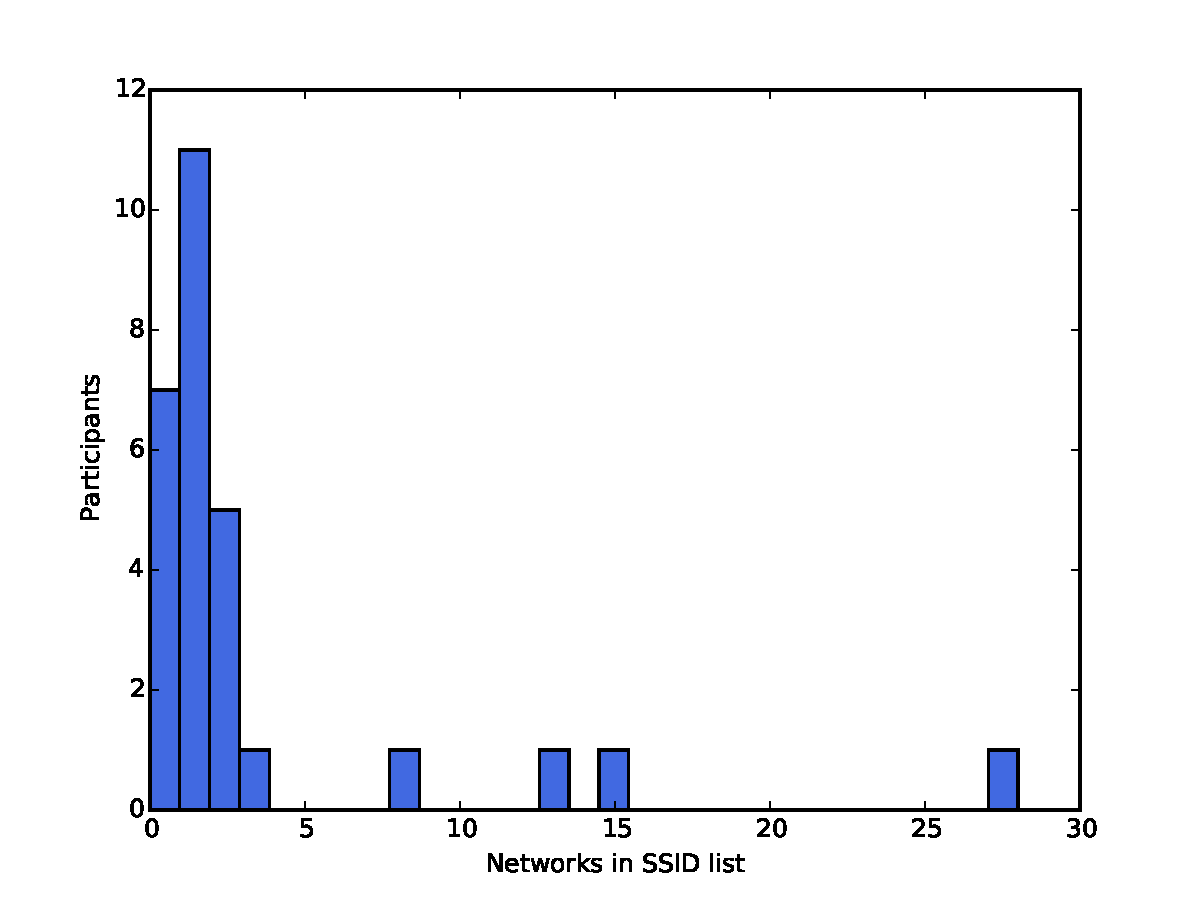
\includegraphics[width=\columnwidth]{hist.pdf}
\caption{Number of participants with each SSID list size}
\end{figure}

\section{Social Network Analysis}
\begin{figure*}
\centering
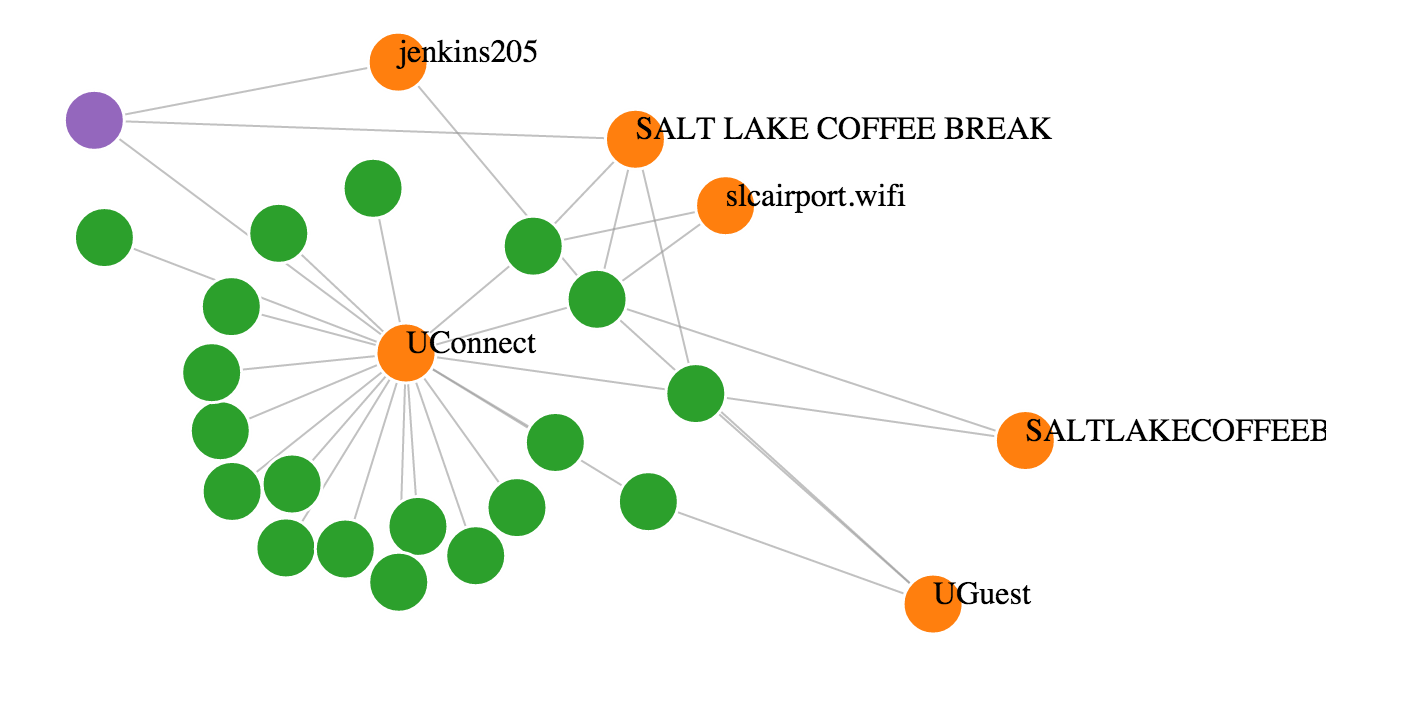
\includegraphics[scale=.5]{graph.png}
\caption{\textsf{Social network graph}}
\end{figure*}

\section{Participant Survey}
We asked our participants to complete a survey after viewing their personalized social network graph.


\section{Future Work}

\section{Conclusion}







\end{document}